\documentclass[../poma-notes.tex]{subfiles}

\begin{document}

\newpage
\subsection*{The Continuity of Derivatives}

我们已经见到了 [Example 5.6 (b)] 中一个函数 $f$ 可能有一个导数 $f'$ 存在于任何点,但是在某些点并不连续。然而,并不是所有函数都有导数。
特别是,存在于区间中每一点的导数与区间上连续的函数有一个重要的共同性质:假定的中间值(相较于 Theorem 4.23)。准确的称述如下:

\begin{theorem}
  Suppose $f$ is a real differentiable function on $[a, b]$ and suppose $f'(a) < \lambda < f'(b)$. Then there is a
  point $x \in (a, b)$ such that $f'(x) = \lambda$.
\end{theorem}

同样的结果对 $f'(a) > f'(b)$ 也成立。

\begin{proof}
  令 $g(t) = f(t) - \lambda t$。那么 $g'(a) < 0$,那么对于某些 $t_1 \in (a,b)$ 有 $g(t_1) < g(a)$,且 $g'(b) > 0$。因此
  $g$ 在 $[a, b]$ 上某点 $x,\ a<x<b$ 可达极小值(Theorem 4.16)。根据 Theorem 5.8,$g'(x) = 0$。因此 $f'(x) = \lambda$。
\end{proof}

\begin{anote}
  \textbf{定理}:设 $f$ 是 $[a, b]$ 上实值可微函数,设 $f'(a) < \lambda < f'(b)$,那么必有一点 $x \in (a, b)$ 使 $f'(x) = \lambda$。

  证明中第一步的假设 $g(t) = f(t) - \lambda t$ 很关键,其构造的原理是根据定理中 $f'(a) < \lambda < f'(b)$ 该假设而来。

  \begin{align*}
    \begin{split}
      \because g(t) &= f(t) - \lambda t \\
      \therefore g'(t) &= \frac{(f(t) - \lambda t) d}{d t} \\
      &= f'(t) - \lambda \\
      \because f'(a) &< \lambda < f'(b) \\
      \therefore g'(a) &= f'(a) - \lambda \\
      & < 0
    \end{split}
  \end{align*}

  这里的 $g'(a) < 0$ 代表 $g$ 在 $a$ 处递减,那么在 $(a, b)$ 中一定存在一个 $t_1$ 满足 $g(t_1) < g(a)$;同理,
  $g'(b) = f'(b) - \lambda > 0$ 说明在 $(a, b)$ 中一定存在一个 $t_2$ 满足 $g(t_2) < g(b)$。

  那么根据 Theorem 4.16 的:$\mathbf{f}$ 是紧度量空间 $X$ 上的连续函数,且 $M = \sup_{p\in X}f(p),\ m = \inf_{p\in X}f(p)$,
  那么一定存在 $r,\ s \in X$ 使得 $f(r) = M,\ f(s) = m$。

  而 $g$ 为两个连续函数之差,其本身也是连续函数,那么其也满足 Theorem 4.16,即 $g$ 具有最大下确界($m = \inf_{p\in X}f(p)$);
  换言之,在 $[a, b]$ 中存在某个点 $x,\ a < x < b$,使得 $g(x)$ 为最小值。

  又根据 Theorem 5.8 的:定义在 $[a,b]$ 上的 $f$;如果 $f$ 在 $x \in (a,b)$ 上具有局部最小值,且 $f'(x)$ 存在,那么 $f'(x)=0$。

  可知 $g'(x) = 0$,那么 $g'(x) = f'(x) - \lambda = 0$ 可得 $f'(x) = \lambda$。
\end{anote}

\begin{corollary}
  If $f$ is differentiable on $[a, b]$, then $f'$ cannot have any simple discontinuities on $[a, b]$.
\end{corollary}

\begin{anote}
  如果 $f$ 在 $[a, b]$ 上可微,那么 $f'$ 在 $[a, b]$ 上不能有简单间断。但是 $f'$ 可能有用第二类间断。

  可见 \href{https://en.wikipedia.org/wiki/Darboux%27s_theorem_(analysis)}{Darboux's theorem}。
\end{anote}

根据此\href{https://math.stackexchange.com/a/423279/1183566}{链接}给出的函数可导,而导数不连续的情况:

\newblock

\textbf{基础案例}

一个可导函数:

\begin{align*}
  f(x) =
  \begin{cases}
    x^2 \sin(\frac{1}{x}) & \text{if $x \ne 0$} \\
    0                     & \text{if $x = 0$}
  \end{cases}
\end{align*}

\begin{figure}[h]
  \centering
  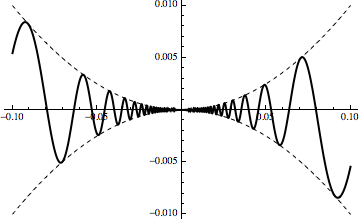
\includegraphics[width=0.5\textwidth]{\subfix{../images/the_continuity_of_derivatives1.png}}
\end{figure}

其导数并不连续:

\begin{align*}
  f'(x) =
  \begin{cases}
    2x \sin(\frac{1}{x}) - \cos(\frac{1}{x}) & \text{if $x \ne 0$} \\
    0                                        & \text{if $x = 0$}
  \end{cases}
\end{align*}

\begin{figure}[h]
  \centering
  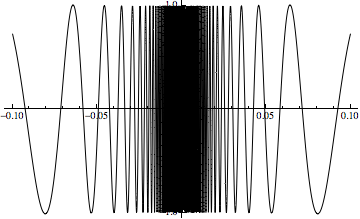
\includegraphics[width=0.5\textwidth]{\subfix{../images/the_continuity_of_derivatives2.png}}
\end{figure}

\newblock

\textbf{两点案例}

一个在 $\mathbb{R}$ 上连续的可导函数(除开两点):

\begin{align*}
  f(x) =
  \begin{cases}
    x^2(1-x)^2\sin(\frac{1}{\pi x(1-x)}) & \text{if $0<x<1$} \\
    0                                    & \text{else}
  \end{cases}
\end{align*}

该 $f$ 与 $f'$ 如图所示:

\begin{figure}[h]
  \centering
  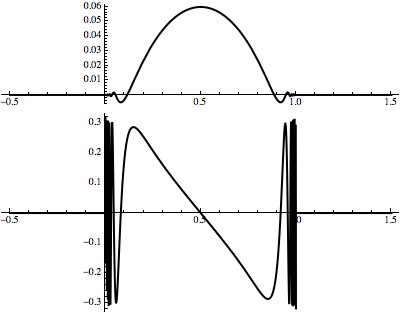
\includegraphics[width=0.5\textwidth]{\subfix{../images/the_continuity_of_derivatives3.png}}
\end{figure}

\end{document}
